\subsection{Emotion Recognition Chain} \label{emotion-recogniton-chain-subsec}

\todo[inline]{Verantwortlich: Artur \\
- ERC Bild ändern (5 statt 4 Schritte)}

Die Emotion Recognition Chain (ERC) besteht aus fünf Hauptschritten: 
Datenerfassung, Vorverarbeitung, Segmentierung, Merkmalsextraktion und Klassifizierung (vgl. Abb. \ref{fig:erc}).
In den folgenden Unterkapiteln wird für jeden Schritt eine allgemeine Erklärung gegeben. \\


\begin{figure}[h]
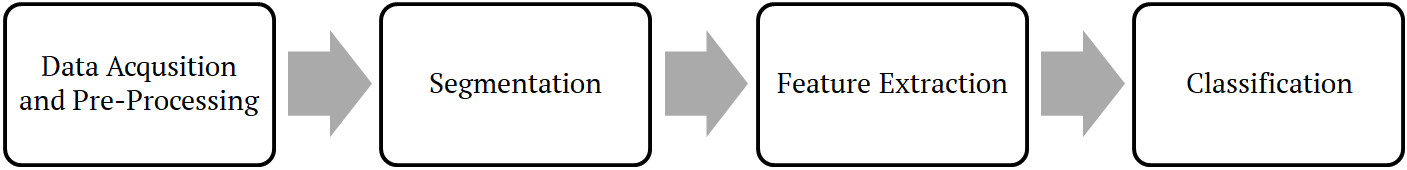
\includegraphics[width=\textwidth]{Images/erc.png} 
\vspace{-0.3cm} 
\caption[Emotion Recognition Chain]{Emotion Recognition Chain: Zeitreihen-Datensätze werden von tragbaren Sensoren aufgenommen (Datenerfassung) und vorverarbeitet (Vorverarbeitung). Die Daten werden dann in Segmente unterteilt (Segmentierung), aus denen Merkmale extrahiert werden (Merkmalsextraktion). Mit den gewonnenen Merkmalen wird schließlich ein Klassifikator trainiert und anschließend dessen Ergebnisse bewertet (Klassifikation).}
\label{fig:erc} 
\end{figure}
%\vspace{0.5cm}


% Unterkapitel
\subsection{Datenerfassung} \label{datenerfassung-1}


In Kapitel \ref{messreihe-1-sec} wurde das verwendete Datenset bereits detailiert beschrieben, sodass hier darauf verzichtet wird. \\

% Unterkapitel 
\subsection{Vorverarbeitung} \label{vorverarbeitung-1}

Wie bereits in Kapitel \ref{vorverarbeitung-0} beschrieben, ist das Ziel der Vorverarbeitung die ”Verbesserung” der Daten f{\"u}r die nachfolgenden Schritte der ERC.
Im Rahmen des ELISE Projektes wurden Normalisierungstechniken auf dem gesamten Datensatz angewendet. 
Wir haben insbesondere die Standardnormalisierung verwendet, welche den Mittelwert der Daten auf Null setzt und die Einheitsvarianz ergibt \cite{grus15}. 
Die Formel f{\"u}r die Standardnormierung lautet:
\begin{equation} 
\Large{ {x'={\frac {x-{\overline {x}}}{\sigma }}} } 
\label{equ:norm} \end{equation} %\vspace{0.5cm}

wobei $ x $ ein Datenpunkt eines Sensorkanales, $ \overline{x} $ ist der Durchschnitt der Gesamtheit f{\"u}r diesen Sensorkanal und $ \sigma $ ist die entsprechende Standardabweichung. \\

% Unterkapitel 
\subsubsection{Segmentation} \label{segmentation-0}

Ziel dieses Schrittes ist es, Teile von Daten zu identifizieren, welche wichtige Informationen über die zu erkennenden Emotionen enthalten. 
Dies geschieht durch Filtern der Daten und Ausschließen von Segmenten, die für das Klassifizierungsproblem nicht relevant sind.
Zusätzlich wird die zu verarbeitende Datenmenge reduziert, indem Segmente eines Zeitfensters fester Größe aus den Daten extrahiert werden.
Diese Vorgeheisweise ist heute in der Praxis besonders wichtig, da sonst hardwarebedingte Einschränkungen die zu verarbeitende Datenmenge begrenzen könnten. \\

% Unterkapitel
\subsection{Merkmalsextraktion} \label{merkmalsextraftion-1}

Wie bereits in Kapitel \ref{merkmalsextraktion-subsubsec} beschrieben, ist das Ziel der Merkmalsextraktion Charakteristiken und Merkmale in den Daten zu finden, die für das
Klassifizierungsproblem von möglichst hoher Relevanz sind. Im Rahmen des ELISE Projektes haben wir verschiedene Vorgehensweisen angewendet. Im den folgenden Unterkapiteln werden diese vorgestellt. \\



% Unterkapitel 
\subsubsection{Handgefertigte Merkmale} \label{hc-features-1}
Der handgefertigten Merkmal Ansatz (enlg. "hand-crafted features approach") besteht in der Berechnung relativ einfacher Merkmale von denen vermudetet wird, dass sie für das Klassifizierungsproblem der Eingangssignale relevant sein können. Diese Vorgehensweise hat den Vorteil des einfachen Aufbaus als auch der relativ geringen benötigten Rechenleistung, wobei potentiell gute Klassifizierungsergebnisse erwarten werden. \\


Obwohl frühere Forschungsarbeiten schon handgefertigte Merkmale zur Emotionserkennung unter mithilfe physiologischer Signale getestet haben (vgl. \cite{martinez_ieee_2013}), wurde dieser Ansatz noch nie für die Erkennung dieser spezifischen Emotionen unter Verwendung dieser Kombination von Sensoren getestet.
Zusätzlich haben wir zuerst handgefertigte Merkmale getestet, um ein Basisergebnis zu liefern, mit der die Ergebnissen der anderen Ansätze vergleichen werden können.
Handgefertigte Merkmale sind in der Regel entweder einfache statistische Werte, Fourier-basierte oder selbstentwickelte Merkmale sein, die aufgrund von Vorkenntnissen der Daten verwendet werden. 
Diese Arbeit wurden statistische, Fourier-basierte und selbstentwickelte Merkmale getestet. \\

\textbf{Statistische Merkmale \\}
Die Tabelle \ref{tab:statistische} fasst die elf verschiedenen und in der Studie verwendeten statistischen Merkmale zusammen. Wir bezeichnen $\mathbf{x} = (x_1, x_2, ...., x_T) $ als Vektor, der die in einem Datenzeitfenster der Länge $T$ enthaltenen Sensorwerte für einen Sensorkanal darstellt. 


\begin{table}[h]
\begin{tabular}{| l | p{12.5cm} |}
\hline
    \textbf{Merkmalname}     &  \textbf{Definition}  \\ \hline
    
    Durchschnitt         & \vspace{0.01cm}
    $ mean(\mathbf{x}) =$ \Large{$\frac{1}{T} \sum_{k=1}^T (x_k) $} \\[0.5cm] \hline 
    
    Standard-Abweichung        & \vspace{0.01cm}
    $ \sigma(\mathbf{x}) =$ \Large{$ \sqrt{ \frac{1}{T} \sum_{k=1}^{T}{(x_k - \mu)^{2}} } $ } \\[0.5cm] \hline
    
    Maximum                   & \vspace{0.01cm}
    $ max(\mathbf{x}) = \max(x_{1},x_{2},\dots ,x_{T}) $
    \\[0.5cm] \hline
    
    Minimum                   & \vspace{0.01cm}
    $ min(\mathbf{x}) = \min(x_{1},x_{2},\dots ,x_{T}) $
    \\[0.5cm] \hline
    
    Amplitude                 & \vspace{0.01cm}
    $ A(\mathbf{x}) = max(\mathbf{x}) - min(\mathbf{x}) $ 
    \\[0.5cm] \hline
    
    25/50/75\% Perzentil      & Wert einer Menge, unter dem 25/50/75\% der Werte aus der Menge fallen. \\ \hline
    
    Interquartiler Bereich    & Differenz zwischen dem 75. und 25. Perzentil.
    \\ \hline
     
    Schräge                   & \vspace{0.01cm}
    $ \gamma _{1}(\mathbf{x}) = \operatorname{E}$ \Large{$\left[\left({\frac {X-\mu }{\sigma }}\right)^{3}\right]$ \normalsize{$=$} ${\frac {\mu _{3}}{\sigma ^{3}}}$ \normalsize{$=$} ${\frac {\operatorname {E} \left[(X-\mu )^{3}\right]}{ (\operatorname {E} \left[(X-\mu )^{2}\right])^{3/2}}}$ \normalsize{$=$} ${\frac {\kappa _{3}}{\kappa _{2}^{3/2}}} $} \vspace{0.2cm}
    \\[0.3cm] \hline
     
    Kurtosis                  & \vspace{0.01cm}
    $ \operatorname {Kurt}[\mathbf{x}] = \operatorname{E} $ \Large{$\left[\left({\frac {X-\mu }{\sigma }}\right)^{4}\right]$ \normalsize{$=$} ${\frac {\mu _{4}}{\sigma ^{4}}}$ \normalsize{$=$} ${\frac {\operatorname {E} [(X-\mu )^{4}]}{(\operatorname {E} [(X-\mu )^{2}])^{2}}} $} \vspace{0.2cm}
    \\[0.3cm] \hline
\end{tabular} 
\caption{Statistische Merkmale, die im Rahmen des ELISE-Projektes verwendet wurden. } \label{tab:statistische}
\end{table} 


\textbf{Fourier-basierte Merkmale \\}
\todo[inline]{Artur: \\
- Muss ich noch schreiben $\rightarrow$ Warten auf Julian's Antwort. \\}


\textbf{Selbstentwickelte Merkmale \\}
Es wurden zwei eigene Merkmale definiert: Nulldurchgang (engl. "zero crossing") und Anzahl der Spitzen (engl. "number of peaks"). Im Folgendem werden diese beiden Merkmale detailiert beschrieben. \\

Das Nulldurchgang-Merkmal zählt die Häufigkeit, mit der das Signal eines Sensorkanals in einem Zeitfenster die Nulllinie überschreitet.
Alle Sensorsignale wurden durch Normierung verarbeitet (vgl. Kapitel xxx) und damit wurden alle Mittelwerte auf Null zentriert.
Um zu vermeiden, dass Rauschen entlang der Nulllinie in dem Merkmal gezählt wird, wird nur ein Nulldurchgang in einer bestimmten Zeitspanne gezählt. \\


Das Spitzenzähler-Merkmal bestimmt die Anzahl von loklanen Hochpunkten im Zeitsignal.
Alle lokalen Maximen sind durch einen Onset (Startpunkt), eine Spitze und einen Offset (Endpunkt) gekennzeichnet (vgl. Abbildung \ref{fig:peaks}). 
Jedes Vorkommen einer Onset/Offset-Paarung wird hierbei als Spitze gezählt.
Onsets, Spitzen und Offsets werden durch die folgenden Operationen identifiziert \cite{BSc_Gouverneu}:

\begin{itemize} %[noitemsep]
  \item Ein Onset wird bestimmt, wenn der Wert des Signals an diesem Punkt nicht negativ ist und die Differenz zwischen ihm und dem nächsten größer als ein vordefinierter Schwellenwert (engl. "threshold") ist.

  \item Ein Offset wird bestimmt, wenn der Wert des Signals kleiner als der Wert des zuletzt gesetzten Onsets ist.

  \item Das lokale Maximum zwischen einem Onset und Offset wird als Spitze bezeichnet.
\end{itemize} \vspace{0.2cm}


\begin{figure}[h] \centering{
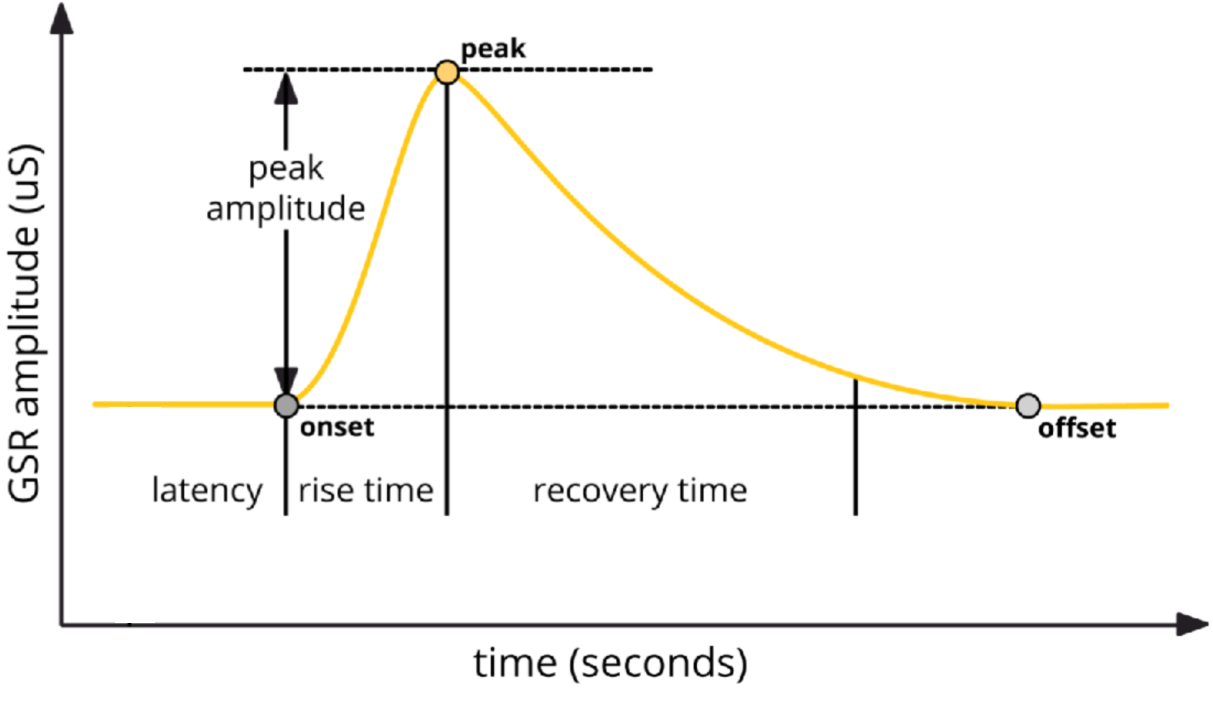
\includegraphics[width=11cm]{Images/peaks.png}}
\caption{ Spitzenzähler: Onset (Startpunkt), Spitze und Offset (Endpunkt). Jedes Paar von Onset/Offset erhöht die Anzahl der Spitzen um eins.} 
\label{fig:peaks} \end{figure} \vspace{0.5cm}


Jedes handgefertigte Merkmal wird auf einem Zeitfenster von Daten für jeden Sensorkanal unabhängig voneinander angewendet. 
Jedes Zeitfenster ist daher 117 Merkmalen zugeordnet (9 Sensorkanäle multipliziert mit 13 Merkmalen). \\





% Unterkapitel 
\subsubsection{Codebook Approach} \label{ca-1}


Die bisherige Methodik mit handgefertigten Merkmalen ist klassisch für den überwachten Lernansatz. 
Es existieren aber auch einige Nachteile. 
Das Hauptproblem besteht darin, dass nicht sichergestellt werden kann, dass die gewählten Merkmale die besten Klassifizierungsergebnisse erzielen. Damit besteht immer die Gefahr, dass möglicherweise andere Merkmalen bessere Ergebnisse liefern würden, diese handgefertigten Merkmale aber die  nicht gefunden wurden. Dieses Risiko besteht insbesondere bei der physiologischen Signalverarbeitung zur Emotionserkennung, wo die Struktur der Daten noch recht unbekannt und allgemein komplex ist. 
Eine weitere Schwierigkeit besteht darin, relevante selbstentwickelte Features ohne Expertenwissen über die Daten zu finden.
Darüber hinaus wurden noch keine gut funktionierenden State-of-the-Art handgefertigten Merkmale identifiziert.
Aus diesen Gründen ist es interessant halbautomatische und unüberwachter Ansätze der Merkmalsextraktion zu verwenden und zu testen. \\


K. Shirahama et al. \cite{kimiaki_codebook_approach_2016} schlugen eine unüberwachte Merkmalsextraktionsmethode namens Codebook Approach (CA) vor, um Merkmale aus 1D-Zeitreihensignalen zu erzeugen.
Der CA hat den Vorteil, dass formbasierte Merkmale gefunden werden können, die für das Problem der Emotionserkennung relevant sind, aber weder offensichtlich noch leicht als Mensch zu interpretieren sind. 
Der CA besteht aus drei Schritten, die in den folgenden Abschnitten erläutert werden: Codebuchkonstruktion (engl. "codebook construction"), Codewortzuordnung (engl. "codeword assignment") und der anschließenden Klassifizierung. \\


\textbf{Codebuchkonstruktion \\}
Ziel dieses Schrittes ist es, Teilsequenzen (sogenannte "Codewörter") zu bestimmen, die für die 1D-Eingangssensorik charakteristisch sind. 
Dies wird erreicht, indem Zeitfenster aus dem ursprünglichen Datensatz für jeden Sensorkanal unabhängig voneinander nach dem im Kapitel \ref{segmenation-1} definierten Segmentierungsansatz extrahiert werden.
Aus jedem so erhaltenen Zeitfenster der Größe $T$ werden kleinere Segmente der Größe $\alpha$ unterteilt.
Ein Clustering-Algorithmus wird dann auf die Menge der Segmente $\alpha$ angewendet, um Clusterzentren zu finden.
Nach der Konvergenz werden die Clusterzentren als Codewörter betrachtet und zum Aufbau einer Sammlung von Codewörtern mit dem Namen ``Codebuch'' verwendet, wie in Abbildung \ref{fig:ca_construction} aus \cite{kimiaki_codebook_approach_2016} dargestellt. 
Die Anzahl der Codewörter (d.h. die Größe des Codebuchs oder die Anzahl der Cluster) ist ein Hyperparameter des Verfahrens. Im Rahmen dieser Arbeit wurde ein k-means Clustering-Algorithmus verwendet, um die Codewörter auf den ELISE-Daten zu erhalten. \\



% Unterkapitel
\subsection{Klassifikation} \label{klassifikation-1}

Wie bereits in Kapitel \ref{grundlagen-klassifikation-0} beschrieben ist das Ziel der Klassifizierung ein Klassifizierungsmodell zu trainieren, das in der Lage ist, Objekte in den Daten in die entsprechende Klasse zuzuordnen. Die Klassen entsprechen hierbei den Emotionen, die erkannt werden sollen: Glück, Langeweile, Frustation und andere (d.h. alle Emotionen, die nicht Glück, Langeweile oder Furstation entsprechen). \\

Als erstes wird der Datensatz in ein Trainigs- und Testset  aufgeteilt. 
Es gibt keine festgelegten Regeln über die Proportionen der Sets. 
Im Allgemeinen wird das Trainingsset aber größer als das Testset gewählt.
Da die Leistungen des Klassifikators jedoch stark von der gewählten Aufteilung abhängen, ist es wichtig, sicherzustellen, dass dieser Schritt richtig durchgeführt wird.
Bei einem Datensatz mit mehreren Probanden empfiehlt sich für die Aufteilung zwischen Trainings- und Testsets die Durchführung einer Leave-One-Subjekt-Out-Cross-Validierung (LOSOCV).
Die Idee besteht darin, $N$ verschiedene Aufteilungen des Datensatzes vorzunehmen, wobei $N$ die Anzahl der Personen ist, die Daten für den Datensatz bereitgestellt haben. 
Für jeden dieser Splits wird der Testset aus den Daten eines Probanden aufgebaut, während die Daten der anderen Probanden das Trainingsset bilden. 
Anschließend wird ein Klassifizierer erstellt und ausgewertet. Dies wird für alle Probanden wiederholt, d.h. $N$ mal.
Die so erhaltenen $N$-Bewertungskennzahlen (eine pro Proband) können dann gemittelt werden, um eine Gesamtbewertung des Modells zu erhalten.
Es ist wichtig zu beachten, dass der LOSOCV-Ansatz bei einer hohen Anzahl von Probanden sehr rechenintensiv sein kann. \\

\begin{figure}[h] \centering{
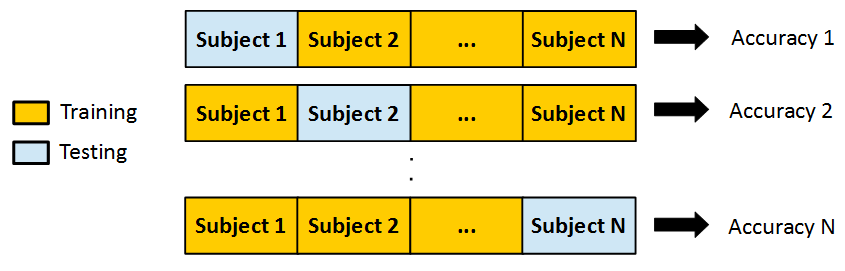
\includegraphics[width=15cm]{Images/LOSOCV.png} 
\caption{ Leave-One-Subjekt-Out-Cross-Validation (LOSOCV): $N$ entspricht der Anzahl der Probanden. Für jeden Split wird ein Testset aus den Daten eines Probanden aufgebaut, während die Daten der anderen Probanden einen Trainingsset bilden. Dieser Vorgang wird für die Daten jedes Probanden durchgeführt. }}
\label{fig:losocv} \end{figure} \vspace{0.5cm}
